\documentclass[a4paper, 14pt]{extarticle}
\usepackage[utf8]{inputenc}
\usepackage[russian]{babel}
\usepackage{longtable, moreverb}
\usepackage{ amssymb, latexsym, amsmath}
\usepackage{graphicx}

\sloppy

\begin{document}
\section{Введение}
Одним из стандартных способов задания функций k\nobreakdash-значной логики являются поляризованные полиномиальные формы (ППФ),
которые также называются обобщенными формами Рида-Мюллера, или каноническими поляризованными полиномами. В ППФ каждая переменная
имеет определенную поляризацию. Длиной полиномиальной формы называется число попарно различных слагаемых в ней. Длиной функции
$F$ в классе ППФ называется наименьшая длина среди длин всех поляризованных полиномиальных форм, реализующих $F$.
Практическое применение ППФ нашли при построении программируемых логических матриц (ПЛМ), сложность ПЛМ
напрямую зависит от длины ППФ, по которой она построена.

Существует быстрый алгоритм построения векторов коэффициентов поляризованных полиномов к-значных функций, полученный
Селезневой С.\,Н. и Маркеловым Н.\,К.:
$$
c^\delta_f(\alpha) = (-1)^{|\alpha|} \sum_{\beta:I(\beta) \subseteq I(\alpha)} \left(  \prod_{a_i \neq 0}b^{k-1-a_i} \right)
f(b_1 - d_1, \dotsc, b_n - d_n), \text{ где}
$$
$k$ - простое число, $f(x_1,\dotsc,x_n) \in P_k^n$, $\delta = (d_1, \dotsc, d_n) \in E_k^n$ - вектор поляризации,
$\alpha = (a_1, \dotsc, a_n)$ - набор из $E_k^n$, $I(\alpha) = \{i:a_i \neq 0\}$, $\beta = (b_1, \dotsc, b_n) \in E_k^n$.

Была необходима программная реализация данного алгоритма, с графическим интерфейсом, что и было проделано в преддипломной
практике.

\newpage

\section{Постановка задачи}
\begin{enumerate}
\item Запрограммированть предлагаемый алгоритм (в статье Селезнева С.Н., Маркелов Н.К. Быстрый алгоритм построения векторов
коэффициентов поляризованных полиномов к-значных функций // Ученые записки Казанского университета. Серия Физико - математические
науки. 2009. 151. \textnumero 2. С. 147-151).
\item Возможности программы: ввод функции как вектора значений, как вектора коэффициентов полинома,
как вектора периода периодической функции.
\item Установить программный продукт на кафедральный компьютер.
\end{enumerate}

\section{Полученные результаты}
Предложенный алгоритм реализован консольной праграммой. Данная программа написана на языке \verb!C++!, и получает параметры
аргементами команндной строки. В программе может обрабатываться функция представленная в одной из трех форм:
\begin{itemize}
\item вектор значений функции,
\item вектор коэффициентов полинома,
\item вектор периода периодической функций.
\end{itemize}
Программа скомпилирована с максимальной оптимизацией, для улучшения производительности.

Интерфейс для работы с пользовтелем написан на языке \verb!perl!, с использованием библиотеки \verb!Tk!.
Интерфейс скрывает от пользовтеля прямую работу с команндной строкой, избавляя от неоходимости запоминать порядок аргументов и от
работы в эмуляторе терминала.
\begin{figure}[t]
\centering
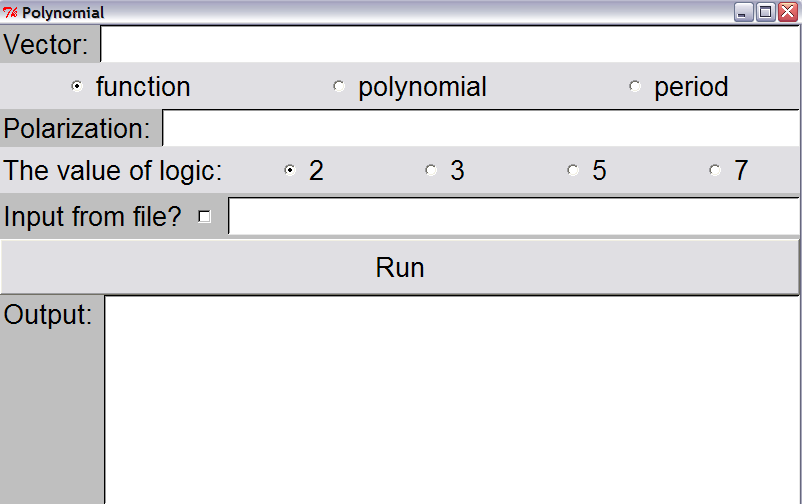
\includegraphics[width=0.95\textwidth]{xp.png}
\caption{Вид интерфейса \label{xp}}
\end{figure}

\newpage

В поле 'Vector' пользовтелю предлагается ввести:
\begin{itemize}
\item вектор значений для обычной функции,
\item вектор коэффициентов полинома, если этот полином имеет не нулевую поляризацию, то через ';' надо ввести поляризации,
для полиномиального представления функции,
\item число переменных и, через пробел, вектор периода, для переодической функции.
\end{itemize}
Далее нужно выбрать соответствующий тип входного представления.
Затем вводится поляризация и выбирается тип логики.

Если пользователь хочет работать с файлами, то нужно поставить 'галочку' в поле 'Input from file', затем через ';' ввести имена:
\begin{enumerate}
\item файла содержащего функции в выбранном представлении,
\item файла с полярицациями (для каждой функции своя поляризация),
\item файла, в который, будет записан результат.
\end{enumerate}
Можно указать имена не всех файлов, тогда недостающая информация будет взята из поля 'Vector' или 'Polarization'.

В конце нужно нажать кнопку 'Run' и в поле 'Output' будет выведен результат.
Результатом будет полином, его длина, а при работе с файлами еще информация(длина, функция и поляризация) о самом длинном
и самом коротком полиноме.

Везде, где вводятся векторы, они могут быть записаны чере пробел, запятую, или подряд идущеми цифрами.

Программа (и реализация алгоритма и интерфейс) установлена на кафедральный компьютер в аудитории 595.
\end{document}
